\section{Implementation, Integration and Test Plan}
As previously illustrated, the System consists of many components that can be divided into the following categories:
\begin{itemize}
	\item \textbf{Frontend components}: Client application 
	\item \textbf{Backend components}: user controller, authorization controller, schedule controller, booking controller, notification controller, feasibility manager, model interface, mail service interface, map service interface, booking service interface and push notification interface
	\item \textbf{External components}: booking, map, mail and notification components provided by third-party services and the DBMS
\end{itemize}
In order to implement, integrate and test the System, a \textit{bottom-up strategy} will be used. In particular, will be first implemented, integrated and tested the components of the same subsystem, then the subsystems will be integrated and tested together in order to verify that the System behaves according to specifications.\\
It has to be noticed that the components of the external subsystem don't need to be tested because the external services are considered reliable. Then, they will be used in place of stubs in order to test the interfaces.\\
Hence, the implementation and integration process will be performed in two levels:
\begin{enumerate}
	\item Implementation and integration of different components of the same subsystem
	\item Integration of different subsystems
\end{enumerate}
For what concerns the first step, component integration of the same subsystem will be applied only for the backend subsystem. More specifically, the component to be integrated and tested together in this category are:
\begin{itemize}
	\item User controller and model interface, forming the \textit{User subsystem}
	\item Authorization controller, model interface and mail service interface, forming the \textit{Auth subsystem}
	\item Notification controller, push notification interface and schedule controller, forming the \textit{Notification subsystem}
	\item Schedule controller, model interface, feasibility manager and map service interface, forming the \textit{Schedule subsystem}
	\item Booking controller, model interface and booking service interface, forming the \textit{Booking subsystem}
\end{itemize}
For the second step the only subsystem integration that will be performed is between the backend and the frontend. The reason of this choice is due to the fact that the frontend and the external subsystems are independent and, as previously said, the external services will be used in place of stubs to test the interfaces but not tested by themselves.\\
Hence, the integrations between the backend subsystems and frontend subsystem that will be performed are:
\begin{itemize}
	\item Client application and User subsystem
	\item Client application and Authorization subsystem
	\item Client application and Schedule subsystem
	\item Client application and Booking subsystem
\end{itemize}
After the application of this procedure, all the subsystems are integrated and tested together.

\subsection{Sequence of Component Integration}
The following diagrams describe the process of implementation, integration and testing. The arrow goes from the used component/subsystem to the component/subsystem that uses it.
\\ \\
\noindent
\textbf{Integration of the backend subsystem}\\ \\
All the components are first implemented and unit tested. Then some of the components are integrated and integration tests will be performed. The integrations are the following:
\begin{figure}[h!]
	\centering
	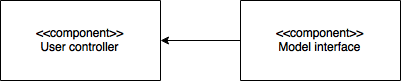
\includegraphics[width=0.5\textwidth]{backend1.png}
	\caption{User subsystem}
\end{figure}
\begin{figure}[h!]
	\centering
	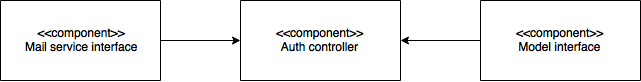
\includegraphics[width=0.8\textwidth]{backend2.png}
	\caption{Authentication subsystem}
\end{figure}
\begin{figure}[h!]
	\centering
	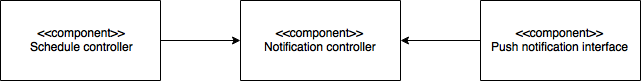
\includegraphics[width=0.8\textwidth]{backend3.png}
	\caption{Notification subsystem}
\end{figure}
\newpage
\begin{figure}[h!]
	\centering
	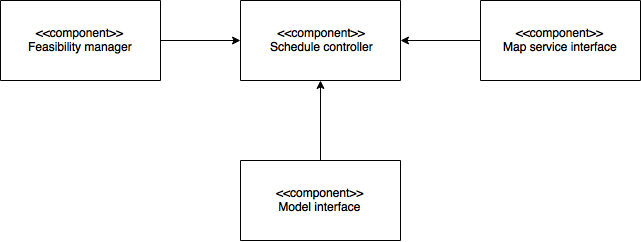
\includegraphics[width=0.8\textwidth]{backend4.png}
	\caption{Schedule subsystem}
\end{figure}
\begin{figure}[h!]
	\centering
	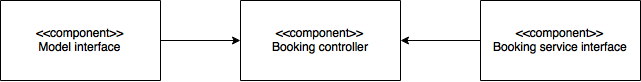
\includegraphics[width=0.8\textwidth]{backend5.png}
	\caption{Booking subsystem}
\end{figure}

\noindent
\textbf{Integration of backend and frontend}\\ \\
Once all the components of the backend are fully implemented and tested, the frontend will be integrated and tested with the backend. In particular, the subsystems to be integrated with the \textit{Client subsystem} are the \textit{User subsystem, Auth subsystem, Schedule subsystem} and \textit{Booking subsystem}.
\newpage
\begin{figure}[h!]
	\centering
	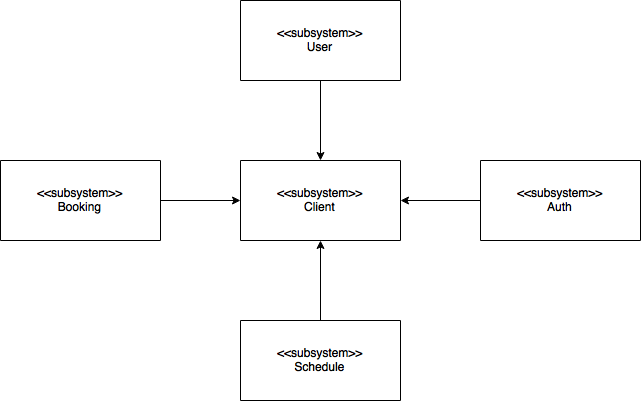
\includegraphics[width=0.8\textwidth]{frontbackend1.png}
	\caption{Client subsystem integration}
\end{figure}

\noindent
\textbf{System integration}\\ \\
At the end of the procedure explained before, the \textit{Frontend}, \textit{Backend} and \textit{External Subsystems} are integrated and tested together.
\begin{figure}[h!]
	\centering
	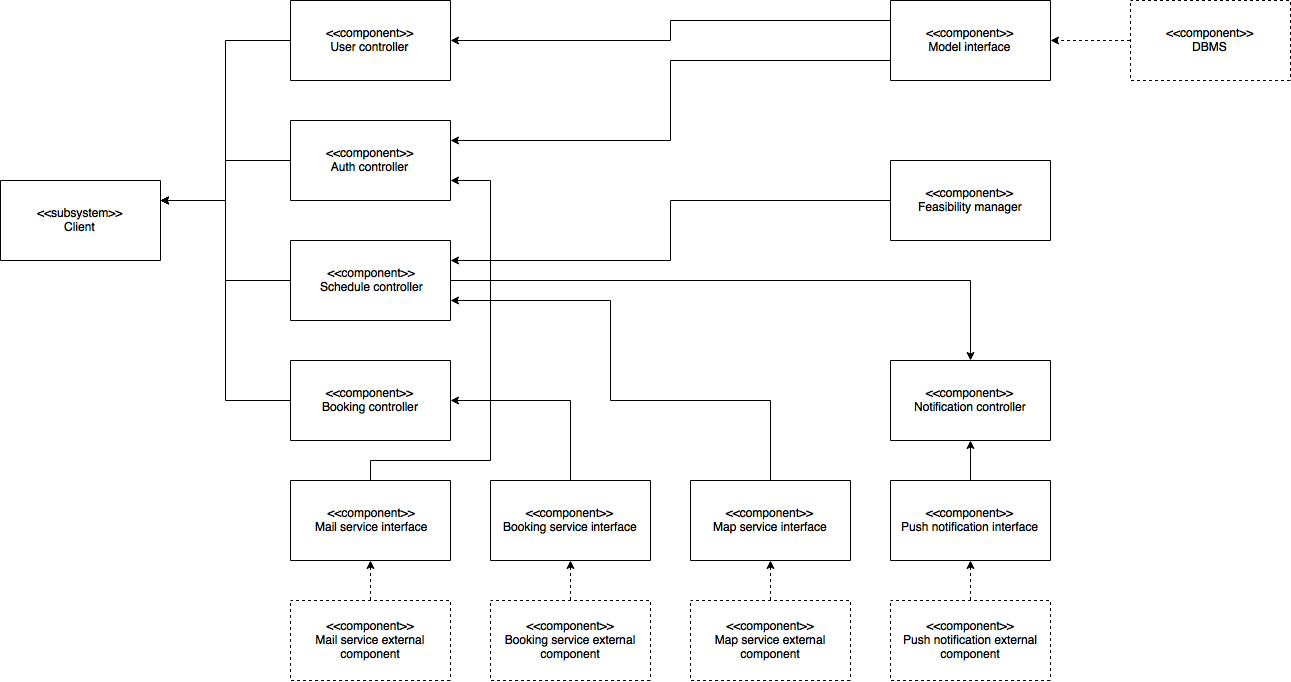
\includegraphics[width=\textwidth]{backendexternal7.png}
	\caption{Subsystems integration}
\end{figure}